\section{Introduction}
\label{sec:intro}

Crowdsensing has become more and more popular, one reason is that mobile devices are becoming increasingly powerful with media processing capable. In fact, a phone has been a small media center, storing all kinds of media files, like videos, images and so on. Consider a scenario that we need to get some photos or video clips of specified information from the mobile phone directly and realtime, because we can't store all the media in the cloud and not necessary to do so, the intuition for this is to search contents on phone over wireless connection. So we want to build a query server that process queries and get the requested photos from the phones. Instead storing all the media files on the server, we can store the meta data of the media files on it. Here, we need the phones to process the media files and get their meta data first and upload to the query server.

Our work focuses on the design of this query service architecture. Let's discuss the query first, sometimes, one may need to have more knowledge of what happened in certain time and place. So time interval and location should be an essential aspect in queries. And in some scenarios, like army, they want to know whether there exist events in specified time and location, such as any person entered building, any car drove through and so on. To thoroughly describe an event there, we include the demands in the query, so we define query as a vector, $\overrightarrow{\mathbf{Q}}$=(time, location, objects, action(objects combination), deadline). After the query server received the queries, then it begins to process the meta-data based on queries. How to find the best fit photos? Since mobile phones' uploading speed is limited and query's deadline is firm, there exists a case that even some photos are qualified, we can't upload all to the server. Here comes another difficulty, how to select from these photos. Our goal is to get as much information for the query, one intuition is to make qualified photos as diverse as possible. For this, we define "similarity" among photos, so we aim to select a subset of photos that satisfy least similarity requirement.

\section{Problem Formulation}
\label{sec:probl}



Next, we will give a detailed problem formulation. System consists of central query server and registered users who are willing to reply the query task assigned by the query server. Whenever comes a query, the central server filters the information with query, and then adopts scheduling algorithm to calculate uploading photos with the photo's meta data. Given the schedule, the central server begins to assign tasks for the phones, and phones response and upload the assigned photos. To make the system model clear, we separate it into 3 parts: Filtering, Network Model and Information Model

First, let's talk about the first step of our system: Filtering. We build "big table" based on the meta data. Objects works as keys, and each column associated with it represents a photos, which contains $(timestamp, location, user_id)$ and gets sorted by timestamp. When the query comes, we search corresponding object rows and refer to the satisfied time range from columns. Next, we further filter these photos with location range. After that, we cluster the qualified photos by user identities, which is the input for the scheduling scheme.

Second, Network Model. After Filtering, we get a bunch of  media files index clustered by user identities. We assume there are $N$ users that own these media files, for user $i$ owns $a_{i}$ files, and each file $j$ has a size of $s_{i,j}$. Each user $i$'s bandwidth is $b_{i}$ and upload files sequentially, besides, they are independent with each other, which means their wireless communication won't affect each other. So in the network side, the scheduling should consider the network conditions in user side, and requires participated user to upload the best subset of files within deadline $T$.

Third, Information Model. Information model is the kernel part for scheduling. Network  gives a constraint for our system,
 so the remaining problem is how to select photos from the qualified photos under the constraint. We define a new term, called ${similarity}$, to describe the relationship between any pair of photos. To make problem clear, we take two files: file $i$ and file $j$ as an example here, the similarity vector ${\overrightarrow{v}_{i,j}}$ is composed by the following elements: time difference ${t_{i,j}}$, location difference ${d_{i,j}}$, object difference ${o_{i,j}}$, color distribution difference ${c_{i,j}}$, trace direction ${tr_{i,j}}$, etc. Since files are owned by different users, then file owner is also an important part for similarity, and we add this information as a binary value in similarity. So now we normalize these elements and define similarity as the weighted sum of these elements. With normalization, the similarity vector can be represented as follows:

 \begin{equation}
\begin{array}{l}
 {\overrightarrow{v}_{ij}} =  \\
 \left( {\frac{{{t_{i,j}}}}{{\mathop {\max }\limits_{i,j} \left( {{t_{i,j}}} \right)}},\frac{{{d_{i,j}}}}{{\mathop {\max }\limits_{i,j} \left( {{d_{i,j}}} \right)}},\frac{{{o_{i,j}}}}{{\mathop {\max }\limits_{i,j} \left( {{o_{i,j}}} \right)}},\frac{{{c_{i,j}}}}{{\mathop {\max }\limits_{i,j} \left( {{c_{i,j}}} \right)}},\frac{{t{r_{i,j}}}}{{\mathop {\max }\limits_{i,j} \left( {t{r_{i,j}}} \right)}}} \right) \\
 \end{array}
 \end{equation}



To quantify the similarity value, we define a weighted sum function for similarity vector, $f_{\overrightarrow{v}_{i,j}}$, which is a numerical value.

\begin{equation}
\begin{array}{l}
 f\left( {{\overrightarrow{v}_{ij}}} \right) = {\alpha _1}\frac{{{t_{i,j}}}}{{\mathop {\max }\limits_{i,j} \left( {{t_{i,j}}} \right)}} + {\alpha _2}\frac{{{d_{i,j}}}}{{\mathop {\max }\limits_{i,j} \left( {{d_{i,j}}} \right)}} +  \\
 {\alpha _3}\frac{{{o_{i,j}}}}{{\mathop {\max }\limits_{i,j} \left( {{o_{i,j}}} \right)}} + {\alpha _4}\frac{{{c_{i,j}}}}{{\mathop {\max }\limits_{i,j} \left( {{c_{i,j}}} \right)}} + {\alpha _5}\frac{{t{r_{i,j}}}}{{\mathop {\max }\limits_{i,j} \left( {t{r_{i,j}}} \right)}} \\
 \end{array}
\end{equation}

in which, $\alpha_{1}+\alpha_{2}+\alpha_{3}+\alpha_{4}+\alpha_{5}=1$, and each $\alpha$'s value is assigned by the query's preference, e.g. if commander prefers location difference, then $\alpha_{1}$ gets more percentage.

Consider the simplest case, each file is of same size and one query scenario. After filtering, we get $N$ photos from $M$ users, each user $i$ owns $a_{i-1}$ photos, that is, $a_{0}+\ldots+a_{M-1}=N$. With the bandwidth and deadline constraint, users can only upload limited qualified files, more precisely, for user $i$, he can upload $s_{i}$ files under the constraint, in which, $s_{i}\leq a_{i}$ and $s_{0}+\ldots+s_{M-1}=K$. The problem now is to select a subset $K$ photos from these $N$ photos, such that:
\begin{equation}
\sum\limits_{i = 0}^{K - 1} {\sum\limits_{j = 0}^{K - 1} {\sum\limits_{{k_i} = 0}^{{s_i} - 1} {\sum\limits_{{k_j} = 0}^{{s_j} - 1} {f\left( {{{\vec v}_{{k_i}{k_j}}}} \right)} } } }
 \end{equation}

 get maximized, in which, $f(\overrightarrow{v}_{k_{i}k_{j}})=0$ if $k_{i}=k_{j}$ and $i=j$.

\section{NP-Completeness and Heuristics}
\label{sec:heuri}

This scheduling optimization is an NPC complete problem. We give a greedy algorithm that may work here. First, sort the $\frac{N(N-1)}{2}$ similarity values. Second, assign each user $i$ a number bucket with capacity $s_{i}$, from the head of the pair queue, fill corresponding bucket with file id if any file hasn't get marked and bucket is not full, until all bucket get full.

\section{System Architecture}
\label{sec:archi}

Till now, we generally describe the system architecture, and Figure~\ref{fig:architecture} shows the architecture
\begin{figure}
\centering 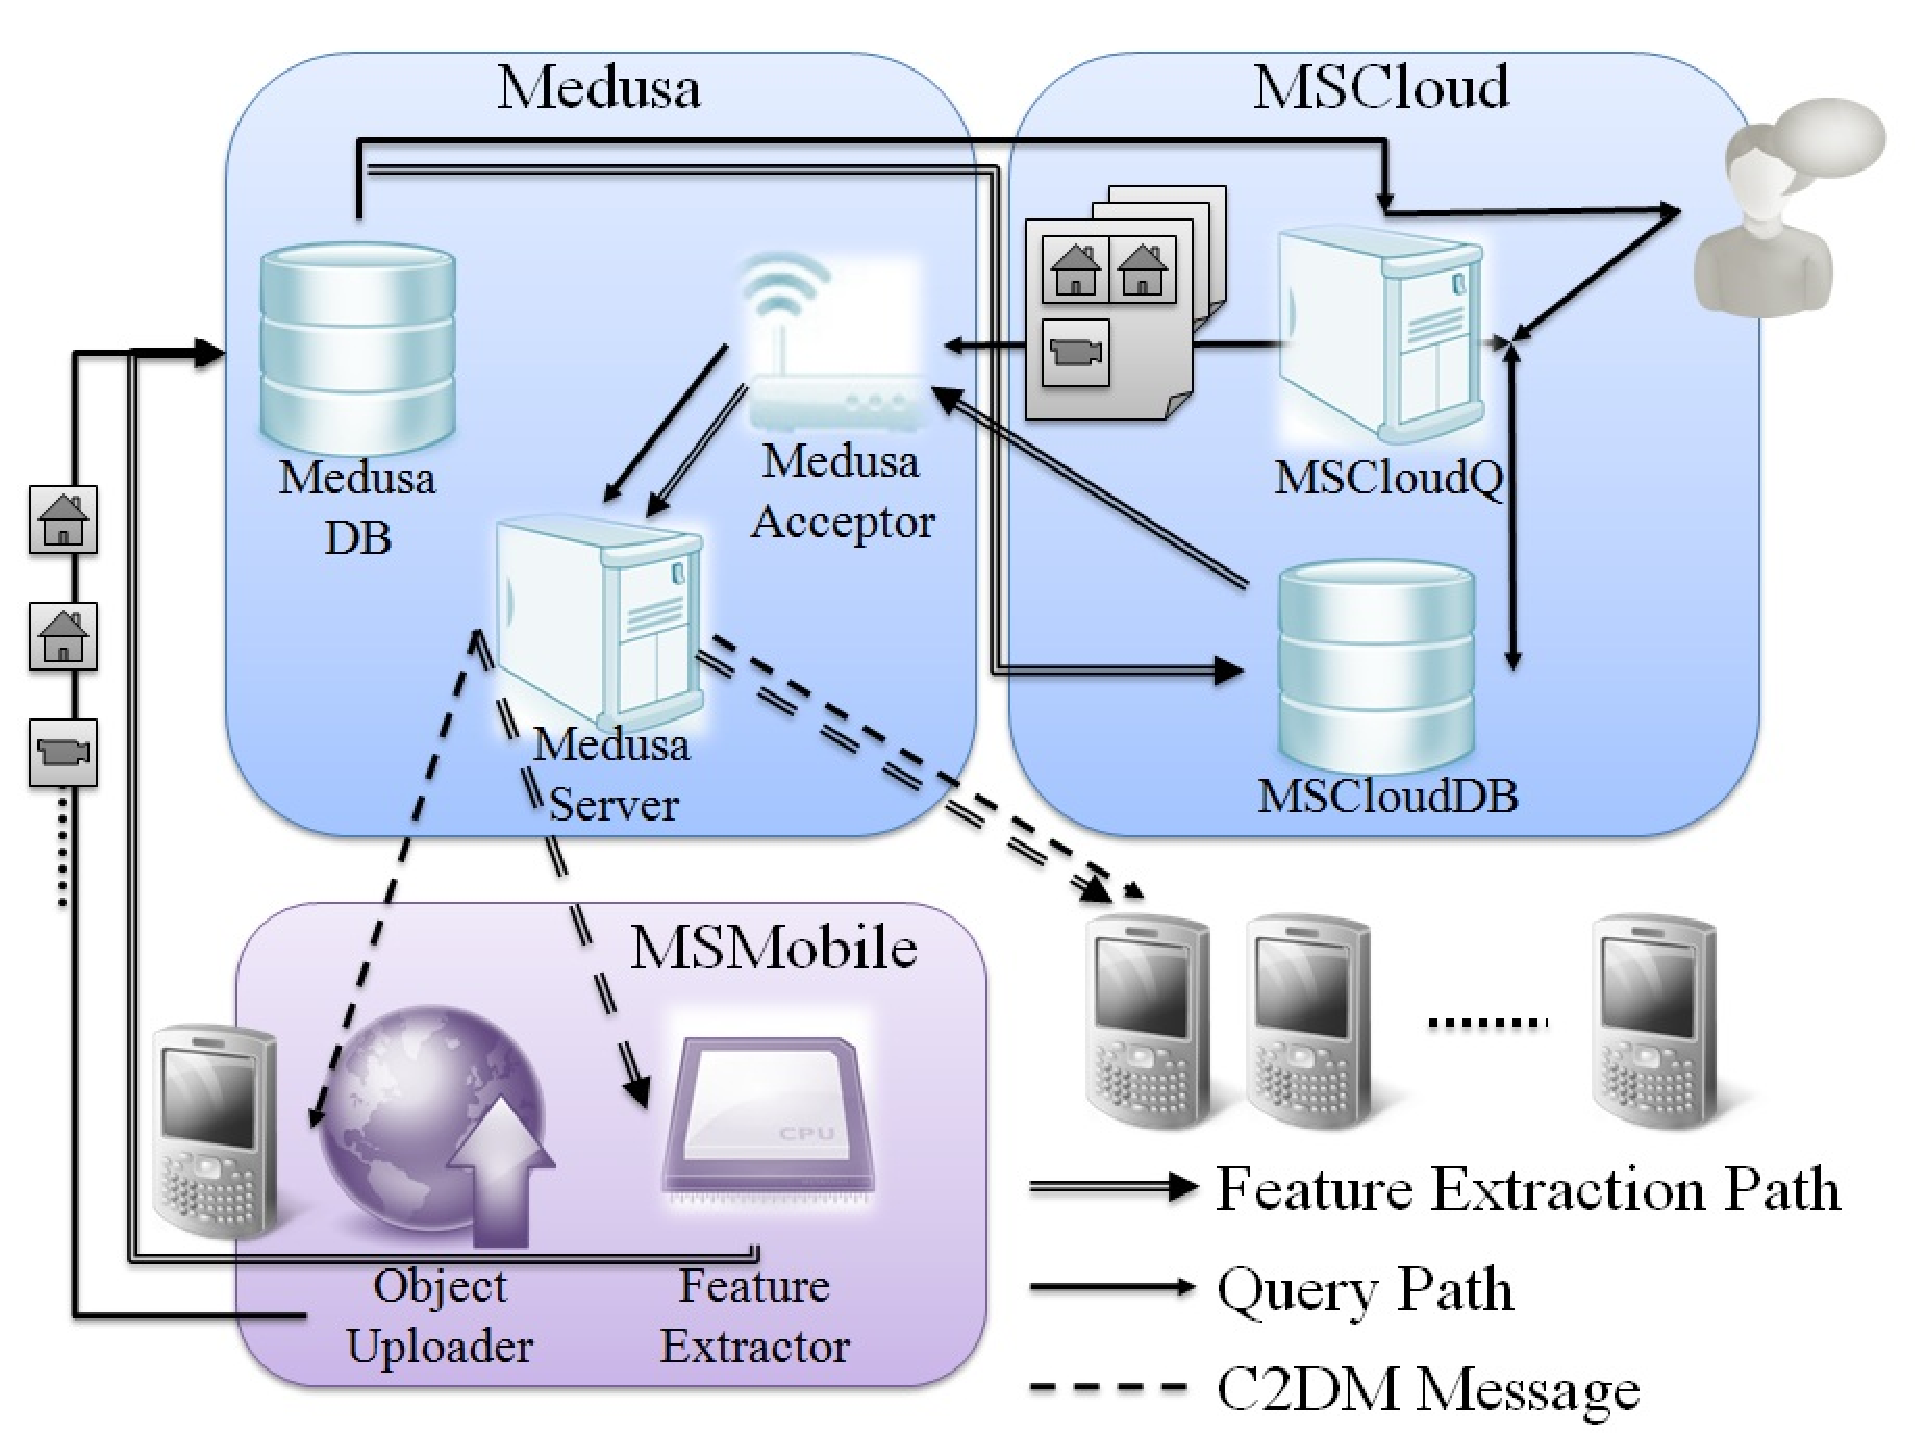
\epsfig{file=pics/architecture.eps, height=1.75in}
%\vspace{-1mm}
\caption{System architecture}
\vspace{-6mm}
\label{fig:architecture}
\end{figure}



\ignore{
In practice, file size varies since we may need to upload different type of media, such as video clips, cropped image or resized image. So the above greedy algorithm may need some modification. Current idea for this problem is to give preference to different file type, and then change the previous number bucket to size bucket so the greedy process is nearly same.

Moreover, queries usually come randomly, which raises another multi-query processing demand for the system. In this situation, we propose a dynamic scheduling adjust algorithm here. To make explanation more clear, we begin with discussion of 2-query overlap scenario, assume the first query time is $[t_{1},t_{2}]$ and second query time is $[t_{3},t_{4}]$, , so the overlapping time is $OL=[max(t_{1},t_{3}),min(t_{2},t_{4})]$, to make discussion simple, we omit the schedule computing time, and add another metric called $rank$ when assign tasks to each user. For the files in the assigned task, we give them a rank, that requires uploading the highest rank file first. The rank is given based on the average similarity, the less similarity, the higher rank, and each file in the rank is associated with a ranking value represents its similarity between other files. Let's come back to the overlap design, during the overlapping time interval $OL$, those who have overlap, should follow the 2 rules: 1. upload overlap files(files that work for both queries), 2. delete from end of 2 ranking lists based on the ranking value, until satisfies  the overlap time consumption. Now, we give a solution to 2 queries scenario, it's easy to generalize to n-query scenario-just find the overlap time interval, and delete end of ranking list until satisfy the requirement.}


